\documentclass[letter,11pt]{scrartcl}
\usepackage{amsmath,amssymb}
\usepackage[amssymb]{SIunits}
\usepackage[T1]{fontenc}
\usepackage[utf8]{inputenc}
\usepackage{standalone}
\usepackage{tikz,pgf,pgfplots}
\usetikzlibrary{decorations.pathmorphing}

\usepackage[margin=20mm]{geometry}
\newenvironment{exercise}[1][Uppgift]{\begin{trivlist} \item[\hskip
    \labelsep {\stepcounter{exerctr}\bfseries #1
      \arabic{exerctr}}]}{\end{trivlist}\vspace{10mm}}

\newcounter{exerctr}
\newcounter{abcctr}[exerctr]

\newcommand{\abc}{\noindent\vspace{1mm}\\ {\bf
    \stepcounter{abcctr}(\alph{abcctr})\ }}
\newcommand{\bbm}{\begin{bmatrix}}
\newcommand{\ebm}{\end{bmatrix}}
\newcommand{\point}[1]{\hfill {\bf (#1p)}\\ \vspace{-5mm}}
\newcommand{\ctrb}{\EuScript{S}}
\newcommand{\Lap}{\mathcal{L}}
\newcommand{\obsv}{\EuScript{O}}
\newcommand{\realdel}[1]{\text{Re}\left\{#1\right\}}
\newcommand{\imagdel}{\text{Im}}
\newcommand{\bC}{\mathbb{C}}
\newcommand{\bR}{\mathbb{R}}
\newcommand{\bmpv}{\begin{minipage}[t]}
\newcommand{\bmps}{\begin{minipage}[t]{45mm}}
\newcommand{\bmpm}{\begin{minipage}[t]{90mm}}
\newcommand{\bmpl}{\begin{minipage}[t]{\textwidth}}
\newcommand{\emp}{\end{minipage}}
\newcommand*{\zethree}{\big(z - \mexp{-3h}\big)}
\newcommand*{\mexp}[1]{\ensuremath{\mathrm{e}^{#1}}}

\newcommand*\circled[1]{\tikz[baseline=(char.base)]{
            \node[shape=circle,draw,inner sep=2pt] (char) {#1};}}

\tikzset{
   ragged border/.style={ decoration={random steps, segment length=1mm, amplitude=0.5mm},
           decorate,
   }
}


\title{Computerized control partial exam 1 (15\%)}
\author{Kjartan Halvorsen}
\date{}

\begin{document}

\maketitle


\begin{description}
\item[Time] September 15 17:30
\item[Place] 4209
\item[Permitted aids] The single colored page with your own notes, table of Laplace transforms, calculator
\end{description}

All answers should be readable and well motivated (if nothing else is written). Solutions/motivations should be written on the provided spaces in this exam. Use the last page if more space is needed.

\begin{center}
{\Large Good luck!} \\
\end{center}

\begin{tabular}{|l|l|}
\hline
\multicolumn{2}{|l|}{\bmpl
Matricula and name
\vspace*{18mm}
\emp}\\
\hline

\end{tabular}


\clearpage
%-----------------------------------------------------------------
\subsection*{The system}
The drawing in figure \ref{fig:apollo-sketch} shows the Apollo Lunar Module (used to put Neil Armstrong and Buzz Aldrin on the moon July 21 1969). The input signal is the thrust of the attitude thrusters. These thrusters causes an angular acceleration of the Lunar Module, which integrated twice gives a change in its orientation $\theta$.  When the Lunar Module makes an angle to the vertical ($\theta \neq 0$) then the main thrusters will give a horizontal force component and thus an acceleration in the $x$-direction. 
\begin{figure}[hbtp]
\begin{center}
  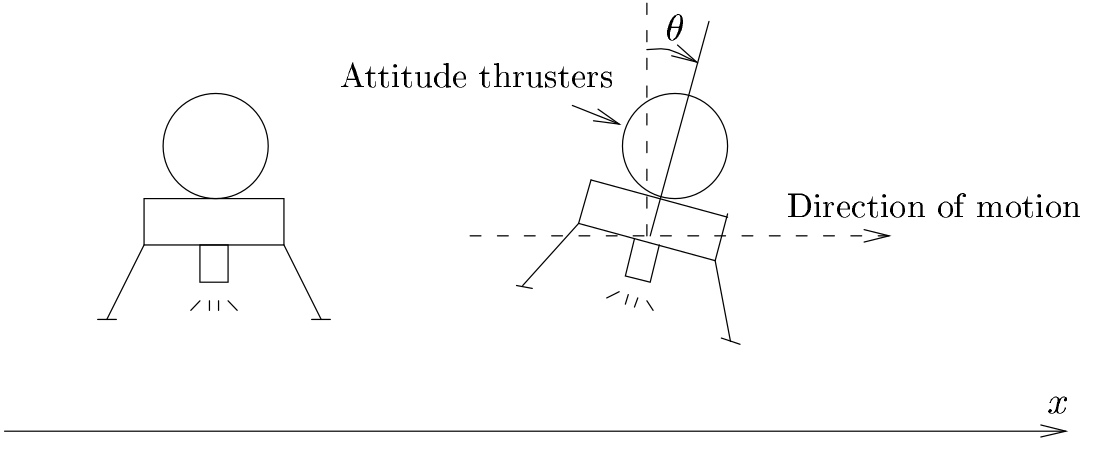
\includegraphics[width=0.6\linewidth]{apollo-2.png}
\end{center}
\caption{Horizontal movement of the Apollo Lunar Module is obtained by tilting the module with respect to vertical.}
\label{fig:apollo-sketch}
\end{figure}

The plant model is described by the block diagram
\begin{center}
  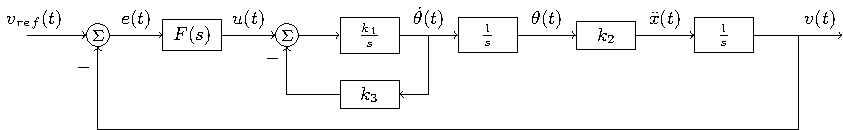
\includegraphics[width=0.9\linewidth]{apollo-block}
\end{center}
Note that the angular velocity is measured using a gyroscope and used in an inner feedback controller. The open-loop transfer function of the plant from the signal $u$ (the control signal to the attitude thrusters) to the  horizontal velocity $v(t)$ is $G(s)=  \frac{k_1k_2}{s^2(s+k_1k_3)}$. For simplicty, assume $k_1=k_2=1$ and $k_3=2$.  


\subsection*{Problem 1}

Discretize the system using zero-order-hold (step-invariant) sampling for arbitrary sampling interval $h$.

What is the relationsship between the poles of the continuous-time system and the poles of the corresponding discrete-time system when doing zero-order-hold sampling?

\noindent
\fbox{
\bmpl
{\bf Derivation and discussion of relationship between the continuous-time and discrete-time poles:}\\
\vspace*{\textheight}
\emp}


\subsection*{Problem 2}

In the rest of the exam, we have $k_3=0$, so there is no inner feedback from the gyro signal.  With a particular choice of sampling period $h$, the following error feedback controller is proposed for the system 
\[ F(z) = K\frac{0.72 z^2 - 1.3 z + 0.60}{z^2 + 0.48 z + 0.10}. \]
\begin{center}
    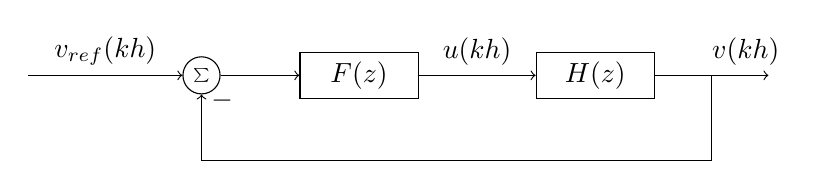
\begin{tikzpicture}[scale = 0.6, node distance=20mm, block/.style={rectangle, draw, minimum width=15mm}, sumnode/.style={circle, draw, inner sep=2pt}]

      \node[block] (plant) {$H(z)$};
      \node[block, left of=plant, node distance=30mm] (controller) {$F(z)$};
      \node[sumnode, left of=controller, node distance=20mm] (refsum) {\tiny $\sum$};
      \node[coordinate, left of=refsum, node distance=22mm] (refinput) {};
      \node[coordinate, right of=plant, node distance=22mm] (output) {};
      
      \draw[->] (refinput) -- node[above] {$v_{ref}(kh)$} (refsum);
      \draw[->] (refsum) -- node[above] {} (controller);
      \draw[->] (controller) -- node[above] {$u(kh)$} (plant);
      \draw[->] (plant) -- node[coordinate] (measure) {} node[above, pos=0.8] {$v(kh)$} (output);
      \draw[->] (measure) -- ++(0,-18mm) -| node[right, pos=0.95] {$-$} (refsum);
     \end{tikzpicture}
   \end{center}

The root locus of the system w.r.t~the gain $K$ is given below
\begin{center}
\begin{tikzpicture}
    \node[anchor=south west,inner sep=0] at (0,0) {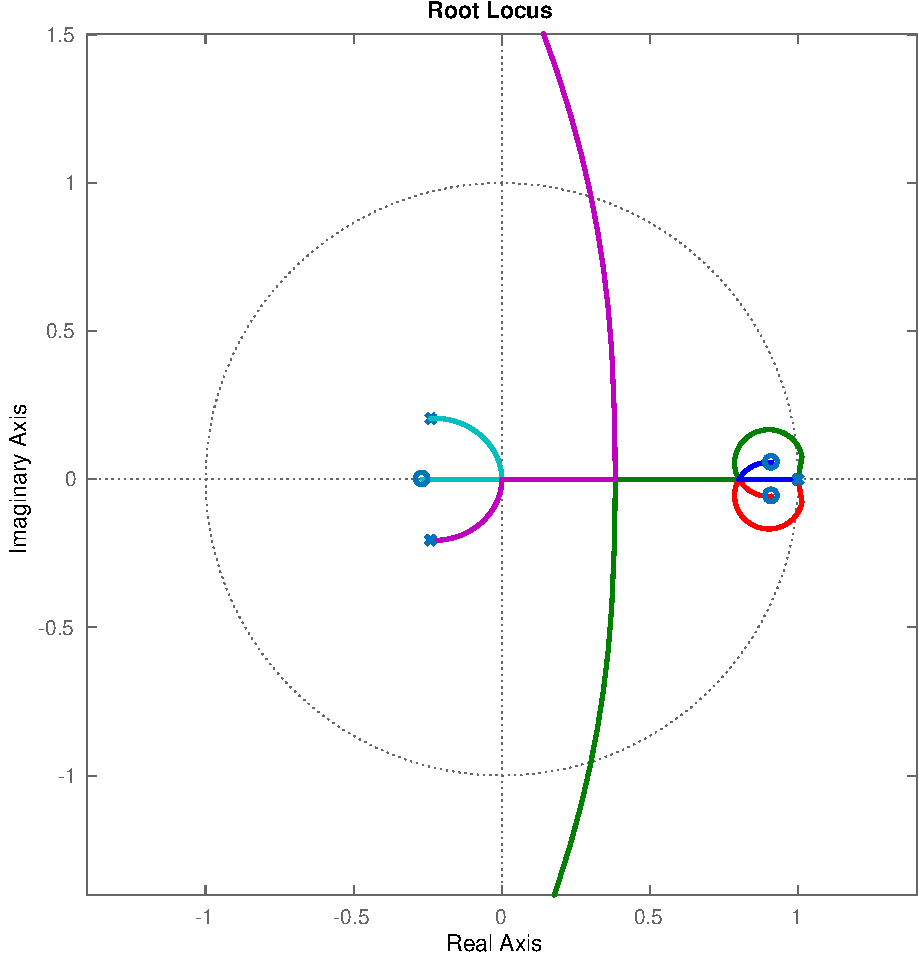
\includegraphics[width=0.6\linewidth]{apollo_rst_rlocus-crop}};
    \node[coordinate, pin={[pin distance=20mm] 10:{$K=2.8$}}] at (6.6,8.45) {};
\end{tikzpicture} 
\end{center}

In figure~\ref{fig:step}, four different closed-loop responses to a step in the reference velocity $v_{ref}$ are shown. The different responses are for four different values of $K$. Identify (and circle) the corresponding step plot for each value of $K$ in the table below. \textbf{Motivate your choice!}

\begin{center}
\begin{tabular}{cl}
\(K\) & Step plot\\\hline
0.08 & A\hspace*{2mm} B\hspace*{2mm} C\hspace*{2mm} D\\
0.3 & A\hspace*{2mm}  B\hspace*{2mm}  C\hspace*{2mm} D\\
1.0 & A\hspace*{2mm} B\hspace*{2mm}  C\hspace*{2mm} D\\
2.5 & A\hspace*{2mm} B\hspace*{2mm}  C\hspace*{2mm} D\\ \hline
\end{tabular}
\end{center}


\begin{figure}[t]
\begin{center}
\begin{tabular}{cc}
A & B\\
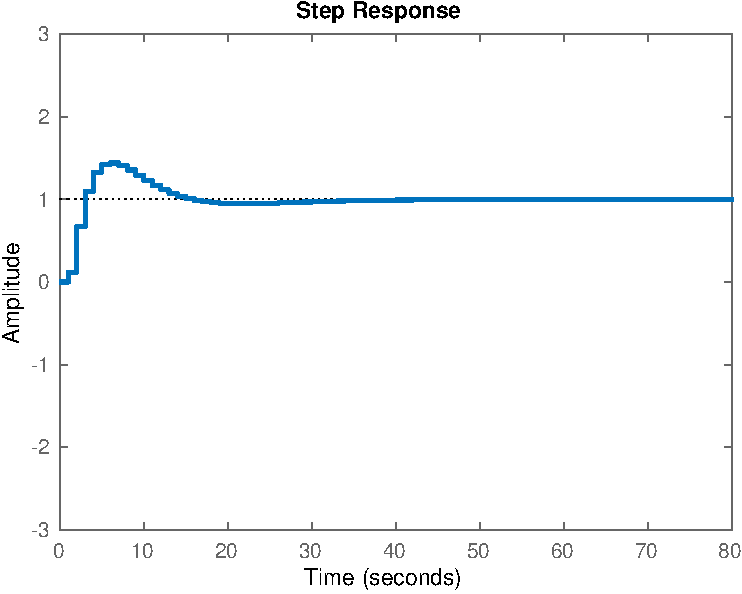
\includegraphics[width=0.4\linewidth]{apollo-step-plot-3-crop}
&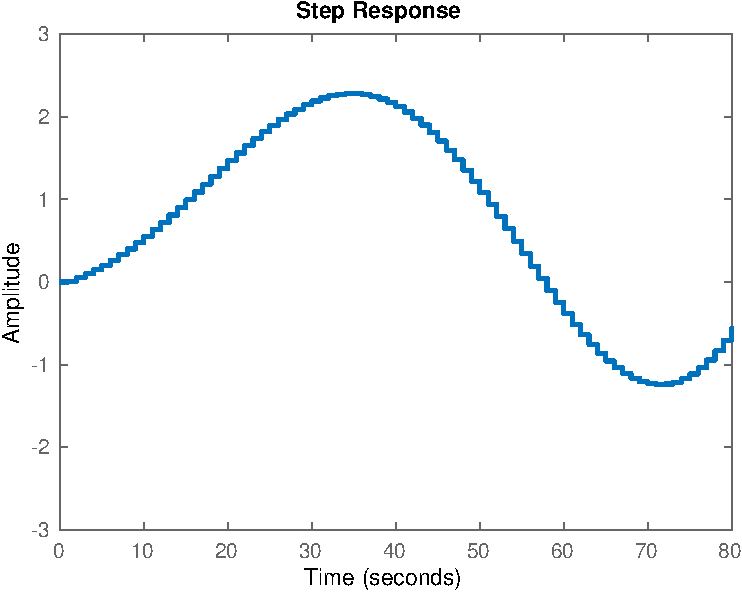
\includegraphics[width=0.4\linewidth]{apollo-step-plot-1-crop}\\
C & D\\
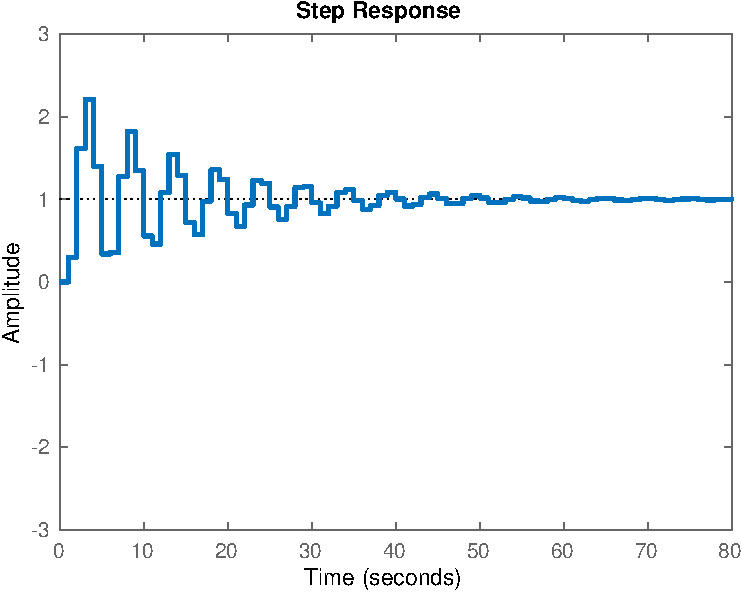
\includegraphics[width=0.4\linewidth]{apollo-step-plot-4-crop}
&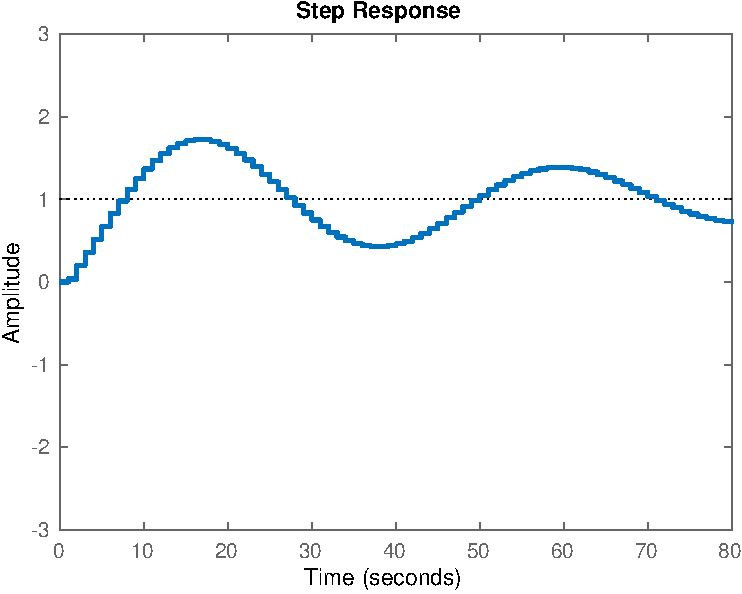
\includegraphics[width=0.4\linewidth]{apollo-step-plot-2-crop}

\end{tabular}
\caption{Step responses for different values of $K$.}
\label{fig:step}
\end{center}
\end{figure}

\noindent
\fbox{
\bmpl
{\bf Motivation:}\\
\vspace*{80mm}
\emp}


%\clearpage

\subsection*{Problem 3}
With the feedback controller of Problem 2, and using $K=1$ we obtain a loop gain $H_o(z)=F(z)H(z)$ whose Bode diagram and Nyquist diagram are given in the figure below. Mark in the figure (both the Bode diagram and the Nyquist diagram) the phase margin and the amplitude margin of the system, and give the corresponding cross-over frequencies.

\begin{center}
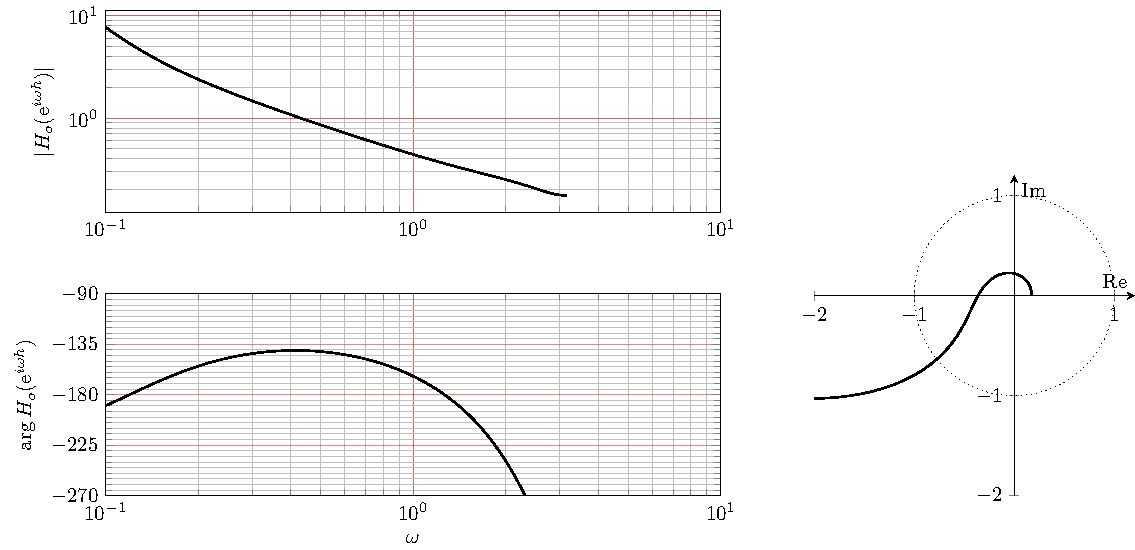
\includegraphics[width=\linewidth]{bode-loop-gain-exc}
\end{center}

\noindent
\fbox{
\bmpl
\begin{tabular}{ll}
Cross-over frequency: & \\[2mm]
Phase margin:&\\[2mm]
Phase cross-over frequency: &\\[2mm]
Amplitude margin: &
\end{tabular}
\emp}


\subsection*{Problem 4 - bonus problem}

What is the sampling period $h$, the Nyquist frequency $\omega_N$ and the sampling frequency $\omega_s$ used in Problem 2 and 3? Is this a reasonable sampling period, in your opinion? Motivation is required! (Bonus problem worth 5p. Full points are possible without answering this question)

\noindent
\fbox{
\bmpl
\begin{tabular}{ll}
Sampling period: & \\[2mm]
Nyquist frequency:&\\[2mm]
Sampling frequency: &\\[2mm]
{\bf Motivation}:\\[80mm]
\end{tabular}
\emp}


% A certain continuous-time transfer function is sampled using zero-order-hold with sampling period $h=1$. The resulting discrete-time system has the poles (crosses) and zero (circle) shown in the figure below.
% \begin{center}
%   \begin{tikzpicture}
%     \pgfmathsetmacro{\bbeta}{0.5*sqrt(2)}
%     \begin{axis} [
%       width=8cm,
%       height=8cm,
%       axis lines=middle,
%       axis line style={->},
%       xtick={-1, 1},
%       ytick={-1,1},
%       yticklabels={$-i$, $i$},
%       %xticklabels={$-b$, -1},
%       xmin=-2,
%       xmax=2,
%       ymin=-2,
%       ymax=2,
%       xlabel=Re,
%       ylabel=Im,
%       ]
      
%       \addplot [ thick,black, mark=x, mark size=4pt, only marks] coordinates { (\bbeta,\bbeta) (\bbeta,-\bbeta)}; 
%       \addplot [ thick,black, mark=o, mark size=4pt, only marks] coordinates { (-1,0) }; 

%       \addplot [ dashed,black, no marks, domain=0:360, samples=800] ( {cos(x}, {sin(x)}); 
%     \end{axis}
%   \end{tikzpicture}
% \end{center}
% *Determine the poles of the continuous-time system.*

% \noindent
% \fbox{
% \bmpl
% {\bf Calculation and answer:}\\
% \vspace*{40mm}
% \emp}






\clearpage

\noindent
{\bf If necessary,} you can continue your solutions on this page. Mark clearly which problem the solution corresponds to.


%\end{document}

%*****************************************************************
%*****************************************************************
\newpage
\setcounter{page}{1}

\section*{Solutions}
\subsection*{Problem 1}
   The transfer function to discretize is \(G(s) = \frac{1}{s^3}\). First calculate the step-response of the system \[Y(s) = G(s)\frac{1}{s} = \frac{1}{s^4} = \frac{1}{3!}\cdot \frac{3!}{s^4}.\] Inverse Laplace-transform gives 
   \[ y(t) = \frac{1}{6} \mathcal{L}^{-1} \left\{\frac{3!}{s^4}\right\} = \frac{1}{6} t^3.\]
   Sampling $y(t)$ gives
   \[ y(kh) = \frac{1}{6} (kh)^3 =  \frac{h^3}{6} k^3 \]
   which has the Z-transform
   \[ Y(z) = \frac{h^3}{6} \cdot \frac{z(z^2 + 4z + 1)}{(z-1)^4}.\]
   Dividing the z-transform of the system response to that of the input (the step) gives
   \begin{align*}
   H(z) &= \frac{Y(z)}{U(z)} = \frac{z-1}{z}Y(z) = \frac{\frac{1}{6}(z^2 + 4z + 1)}{(z-1)^3}.
   \end{align*}

   All the three continuous-time poles are in the orgin. They are mapped to the point $z=1$ in the z-plane by $z=\mathrm{e}^{sh}$ when we use zero-order-hold sampling.

\subsection*{Problem 2}

From the root locus we see that if the gain is $K>2.8$, then the closed-loop system will have two complex-conjugated poles outside the unit circle, and the system will be unstable.  For a gain smaller but close to $K=2.8$ we should observe a response with quite fast osciallations. We know that we have three start-points in $z=1$, and we see that two complex-conjugated branches starting in $z=1$ go outside the unit circle before entering into the stable region. So for low-values of $K$ we should expect poorly damped slow oscillations, or even an unstable system. For intermediate values of $K$, we get poles well inside the unit circle, and so a well-damped response. By this reasoning we arrive at

\begin{description}
\item[$K=0.08$] Slow and oscillatory response. This must correspond to step-response B.
\item[$K=0.3$] Faster response than for $K=0.08$, still maybe oscillatory. This is seen in step-response D
\item[$K=2.5$] Should give two compled-conjugated poles that are fast ($ \omega h \approx 1.2$) and close to the unit circle. We expect fast and poorly damped oscillations with aproximately  five samples per period ($2\pi/1.2 \approx 5$). This must correspond to response C
\item[$K=1$] This leaves the intermediate value $K=1$, which gives a well-behaved and damped response: A.
\end{description}

\begin{center}
\begin{tabular}{cl}
\(K\) & Step plot\\\hline
0.08 & A\hspace*{2mm} \circled{B}\hspace*{2mm} C\hspace*{2mm} D\\
0.3 & A\hspace*{2mm}  B\hspace*{2mm}  C\hspace*{2mm} \circled{D}\\
1.0 & \circled{A}\hspace*{2mm} B\hspace*{2mm}  C\hspace*{2mm} D\\
2.5 & A\hspace*{2mm} B\hspace*{2mm}  \circled{C}\hspace*{2mm} D\\ \hline
\end{tabular}
\end{center}

\subsection*{Problem 3}

\begin{center}
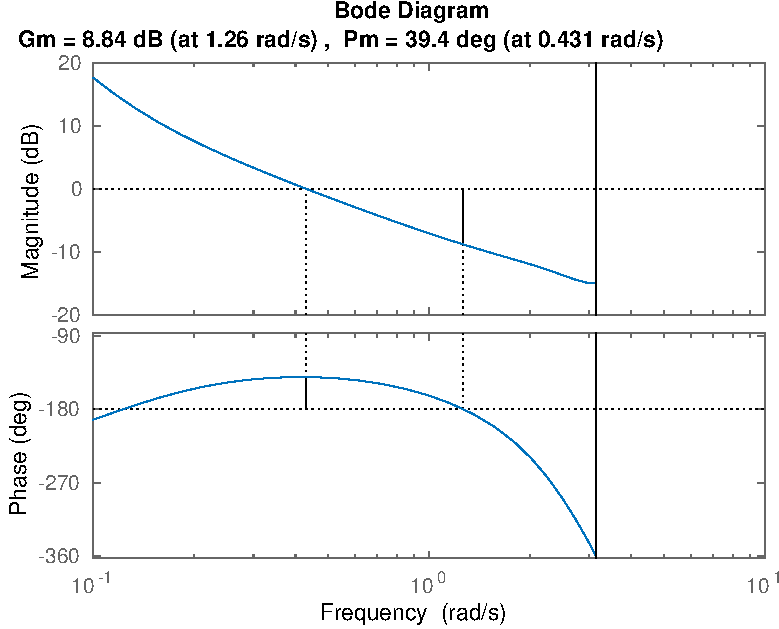
\includegraphics[width=0.7\linewidth]{apollo-rst-margin-crop}
\end{center}
%\end{document}

\subsection*{Problem 4}

There are several ways to find the sampling period $h$. Maybe the easiest is to look at the step-responses in Problem 2. Clearly there are 10 samples per 10 seconds, so $h=\unit{1}{s}$. It can also be seen from the bode diagram of Problem 3 that the plot ends at the frequency $\omega \approx 3.14$, which is the Nyquist frequency. Since $\omega_N h = \pi$, then again we get $h=1$. The sampling frequency (in rad/s) is twice the Nyquist frequency, or $\omega_s = \frac{2\pi}{h} = 2\pi$. 

Is this sampling frequency reasonable? The step-response A in Problem 2 reaches the peak. \unit{1.4}{\meter\per\second} after \unit{6}{\second}. 
which corresponds to an acceleration of approximately 0.2 m/s$^2$.%\unit{0.2}{\meter\per\second\square}. 
This is about 12\% of the gravitational acceleration on the moon
(\unit{1.622}{\meter\per\second\squared}). 
Since the horizontal force comes from the horizontal component of the main thrusters, this means that the module is tilted $\tan^{-1} 0.12 = \unit{7}{\degree}$. Which seems reasonable. On the other hand, in this response we have less than the recommended number of sampling periods per rise time (rule-of-thumb says 4-10). So maybe the sampling period it is a little too long. Half a second is probably better. 

\end{document}
